
% Default to the notebook output style

    


% Inherit from the specified cell style.




    
\documentclass[11pt]{article}

    
    
    \usepackage[T1]{fontenc}
    % Nicer default font (+ math font) than Computer Modern for most use cases
    \usepackage{mathpazo}

    % Basic figure setup, for now with no caption control since it's done
    % automatically by Pandoc (which extracts ![](path) syntax from Markdown).
    \usepackage{graphicx}
    % We will generate all images so they have a width \maxwidth. This means
    % that they will get their normal width if they fit onto the page, but
    % are scaled down if they would overflow the margins.
    \makeatletter
    \def\maxwidth{\ifdim\Gin@nat@width>\linewidth\linewidth
    \else\Gin@nat@width\fi}
    \makeatother
    \let\Oldincludegraphics\includegraphics
    % Set max figure width to be 80% of text width, for now hardcoded.
    \renewcommand{\includegraphics}[1]{\Oldincludegraphics[width=.8\maxwidth]{#1}}
    % Ensure that by default, figures have no caption (until we provide a
    % proper Figure object with a Caption API and a way to capture that
    % in the conversion process - todo).
    \usepackage{caption}
    \DeclareCaptionLabelFormat{nolabel}{}
    \captionsetup{labelformat=nolabel}

    \usepackage{adjustbox} % Used to constrain images to a maximum size 
    \usepackage{xcolor} % Allow colors to be defined
    \usepackage{enumerate} % Needed for markdown enumerations to work
    \usepackage{geometry} % Used to adjust the document margins
    \usepackage{amsmath} % Equations
    \usepackage{amssymb} % Equations
    \usepackage{textcomp} % defines textquotesingle
    % Hack from http://tex.stackexchange.com/a/47451/13684:
    \AtBeginDocument{%
        \def\PYZsq{\textquotesingle}% Upright quotes in Pygmentized code
    }
    \usepackage{upquote} % Upright quotes for verbatim code
    \usepackage{eurosym} % defines \euro
    \usepackage[mathletters]{ucs} % Extended unicode (utf-8) support
    \usepackage[utf8x]{inputenc} % Allow utf-8 characters in the tex document
    \usepackage{fancyvrb} % verbatim replacement that allows latex
    \usepackage{grffile} % extends the file name processing of package graphics 
                         % to support a larger range 
    % The hyperref package gives us a pdf with properly built
    % internal navigation ('pdf bookmarks' for the table of contents,
    % internal cross-reference links, web links for URLs, etc.)
    \usepackage{hyperref}
    \usepackage{longtable} % longtable support required by pandoc >1.10
    \usepackage{booktabs}  % table support for pandoc > 1.12.2
    \usepackage[inline]{enumitem} % IRkernel/repr support (it uses the enumerate* environment)
    \usepackage[normalem]{ulem} % ulem is needed to support strikethroughs (\sout)
                                % normalem makes italics be italics, not underlines
    

    
    
    % Colors for the hyperref package
    \definecolor{urlcolor}{rgb}{0,.145,.698}
    \definecolor{linkcolor}{rgb}{.71,0.21,0.01}
    \definecolor{citecolor}{rgb}{.12,.54,.11}

    % ANSI colors
    \definecolor{ansi-black}{HTML}{3E424D}
    \definecolor{ansi-black-intense}{HTML}{282C36}
    \definecolor{ansi-red}{HTML}{E75C58}
    \definecolor{ansi-red-intense}{HTML}{B22B31}
    \definecolor{ansi-green}{HTML}{00A250}
    \definecolor{ansi-green-intense}{HTML}{007427}
    \definecolor{ansi-yellow}{HTML}{DDB62B}
    \definecolor{ansi-yellow-intense}{HTML}{B27D12}
    \definecolor{ansi-blue}{HTML}{208FFB}
    \definecolor{ansi-blue-intense}{HTML}{0065CA}
    \definecolor{ansi-magenta}{HTML}{D160C4}
    \definecolor{ansi-magenta-intense}{HTML}{A03196}
    \definecolor{ansi-cyan}{HTML}{60C6C8}
    \definecolor{ansi-cyan-intense}{HTML}{258F8F}
    \definecolor{ansi-white}{HTML}{C5C1B4}
    \definecolor{ansi-white-intense}{HTML}{A1A6B2}

    % commands and environments needed by pandoc snippets
    % extracted from the output of `pandoc -s`
    \providecommand{\tightlist}{%
      \setlength{\itemsep}{0pt}\setlength{\parskip}{0pt}}
    \DefineVerbatimEnvironment{Highlighting}{Verbatim}{commandchars=\\\{\}}
    % Add ',fontsize=\small' for more characters per line
    \newenvironment{Shaded}{}{}
    \newcommand{\KeywordTok}[1]{\textcolor[rgb]{0.00,0.44,0.13}{\textbf{{#1}}}}
    \newcommand{\DataTypeTok}[1]{\textcolor[rgb]{0.56,0.13,0.00}{{#1}}}
    \newcommand{\DecValTok}[1]{\textcolor[rgb]{0.25,0.63,0.44}{{#1}}}
    \newcommand{\BaseNTok}[1]{\textcolor[rgb]{0.25,0.63,0.44}{{#1}}}
    \newcommand{\FloatTok}[1]{\textcolor[rgb]{0.25,0.63,0.44}{{#1}}}
    \newcommand{\CharTok}[1]{\textcolor[rgb]{0.25,0.44,0.63}{{#1}}}
    \newcommand{\StringTok}[1]{\textcolor[rgb]{0.25,0.44,0.63}{{#1}}}
    \newcommand{\CommentTok}[1]{\textcolor[rgb]{0.38,0.63,0.69}{\textit{{#1}}}}
    \newcommand{\OtherTok}[1]{\textcolor[rgb]{0.00,0.44,0.13}{{#1}}}
    \newcommand{\AlertTok}[1]{\textcolor[rgb]{1.00,0.00,0.00}{\textbf{{#1}}}}
    \newcommand{\FunctionTok}[1]{\textcolor[rgb]{0.02,0.16,0.49}{{#1}}}
    \newcommand{\RegionMarkerTok}[1]{{#1}}
    \newcommand{\ErrorTok}[1]{\textcolor[rgb]{1.00,0.00,0.00}{\textbf{{#1}}}}
    \newcommand{\NormalTok}[1]{{#1}}
    
    % Additional commands for more recent versions of Pandoc
    \newcommand{\ConstantTok}[1]{\textcolor[rgb]{0.53,0.00,0.00}{{#1}}}
    \newcommand{\SpecialCharTok}[1]{\textcolor[rgb]{0.25,0.44,0.63}{{#1}}}
    \newcommand{\VerbatimStringTok}[1]{\textcolor[rgb]{0.25,0.44,0.63}{{#1}}}
    \newcommand{\SpecialStringTok}[1]{\textcolor[rgb]{0.73,0.40,0.53}{{#1}}}
    \newcommand{\ImportTok}[1]{{#1}}
    \newcommand{\DocumentationTok}[1]{\textcolor[rgb]{0.73,0.13,0.13}{\textit{{#1}}}}
    \newcommand{\AnnotationTok}[1]{\textcolor[rgb]{0.38,0.63,0.69}{\textbf{\textit{{#1}}}}}
    \newcommand{\CommentVarTok}[1]{\textcolor[rgb]{0.38,0.63,0.69}{\textbf{\textit{{#1}}}}}
    \newcommand{\VariableTok}[1]{\textcolor[rgb]{0.10,0.09,0.49}{{#1}}}
    \newcommand{\ControlFlowTok}[1]{\textcolor[rgb]{0.00,0.44,0.13}{\textbf{{#1}}}}
    \newcommand{\OperatorTok}[1]{\textcolor[rgb]{0.40,0.40,0.40}{{#1}}}
    \newcommand{\BuiltInTok}[1]{{#1}}
    \newcommand{\ExtensionTok}[1]{{#1}}
    \newcommand{\PreprocessorTok}[1]{\textcolor[rgb]{0.74,0.48,0.00}{{#1}}}
    \newcommand{\AttributeTok}[1]{\textcolor[rgb]{0.49,0.56,0.16}{{#1}}}
    \newcommand{\InformationTok}[1]{\textcolor[rgb]{0.38,0.63,0.69}{\textbf{\textit{{#1}}}}}
    \newcommand{\WarningTok}[1]{\textcolor[rgb]{0.38,0.63,0.69}{\textbf{\textit{{#1}}}}}
    
    
    % Define a nice break command that doesn't care if a line doesn't already
    % exist.
    \def\br{\hspace*{\fill} \\* }
    % Math Jax compatability definitions
    \def\gt{>}
    \def\lt{<}
    % Document parameters
    \title{LAB01-PR01}
    
    
    

    % Pygments definitions
    
\makeatletter
\def\PY@reset{\let\PY@it=\relax \let\PY@bf=\relax%
    \let\PY@ul=\relax \let\PY@tc=\relax%
    \let\PY@bc=\relax \let\PY@ff=\relax}
\def\PY@tok#1{\csname PY@tok@#1\endcsname}
\def\PY@toks#1+{\ifx\relax#1\empty\else%
    \PY@tok{#1}\expandafter\PY@toks\fi}
\def\PY@do#1{\PY@bc{\PY@tc{\PY@ul{%
    \PY@it{\PY@bf{\PY@ff{#1}}}}}}}
\def\PY#1#2{\PY@reset\PY@toks#1+\relax+\PY@do{#2}}

\expandafter\def\csname PY@tok@w\endcsname{\def\PY@tc##1{\textcolor[rgb]{0.73,0.73,0.73}{##1}}}
\expandafter\def\csname PY@tok@c\endcsname{\let\PY@it=\textit\def\PY@tc##1{\textcolor[rgb]{0.25,0.50,0.50}{##1}}}
\expandafter\def\csname PY@tok@cp\endcsname{\def\PY@tc##1{\textcolor[rgb]{0.74,0.48,0.00}{##1}}}
\expandafter\def\csname PY@tok@k\endcsname{\let\PY@bf=\textbf\def\PY@tc##1{\textcolor[rgb]{0.00,0.50,0.00}{##1}}}
\expandafter\def\csname PY@tok@kp\endcsname{\def\PY@tc##1{\textcolor[rgb]{0.00,0.50,0.00}{##1}}}
\expandafter\def\csname PY@tok@kt\endcsname{\def\PY@tc##1{\textcolor[rgb]{0.69,0.00,0.25}{##1}}}
\expandafter\def\csname PY@tok@o\endcsname{\def\PY@tc##1{\textcolor[rgb]{0.40,0.40,0.40}{##1}}}
\expandafter\def\csname PY@tok@ow\endcsname{\let\PY@bf=\textbf\def\PY@tc##1{\textcolor[rgb]{0.67,0.13,1.00}{##1}}}
\expandafter\def\csname PY@tok@nb\endcsname{\def\PY@tc##1{\textcolor[rgb]{0.00,0.50,0.00}{##1}}}
\expandafter\def\csname PY@tok@nf\endcsname{\def\PY@tc##1{\textcolor[rgb]{0.00,0.00,1.00}{##1}}}
\expandafter\def\csname PY@tok@nc\endcsname{\let\PY@bf=\textbf\def\PY@tc##1{\textcolor[rgb]{0.00,0.00,1.00}{##1}}}
\expandafter\def\csname PY@tok@nn\endcsname{\let\PY@bf=\textbf\def\PY@tc##1{\textcolor[rgb]{0.00,0.00,1.00}{##1}}}
\expandafter\def\csname PY@tok@ne\endcsname{\let\PY@bf=\textbf\def\PY@tc##1{\textcolor[rgb]{0.82,0.25,0.23}{##1}}}
\expandafter\def\csname PY@tok@nv\endcsname{\def\PY@tc##1{\textcolor[rgb]{0.10,0.09,0.49}{##1}}}
\expandafter\def\csname PY@tok@no\endcsname{\def\PY@tc##1{\textcolor[rgb]{0.53,0.00,0.00}{##1}}}
\expandafter\def\csname PY@tok@nl\endcsname{\def\PY@tc##1{\textcolor[rgb]{0.63,0.63,0.00}{##1}}}
\expandafter\def\csname PY@tok@ni\endcsname{\let\PY@bf=\textbf\def\PY@tc##1{\textcolor[rgb]{0.60,0.60,0.60}{##1}}}
\expandafter\def\csname PY@tok@na\endcsname{\def\PY@tc##1{\textcolor[rgb]{0.49,0.56,0.16}{##1}}}
\expandafter\def\csname PY@tok@nt\endcsname{\let\PY@bf=\textbf\def\PY@tc##1{\textcolor[rgb]{0.00,0.50,0.00}{##1}}}
\expandafter\def\csname PY@tok@nd\endcsname{\def\PY@tc##1{\textcolor[rgb]{0.67,0.13,1.00}{##1}}}
\expandafter\def\csname PY@tok@s\endcsname{\def\PY@tc##1{\textcolor[rgb]{0.73,0.13,0.13}{##1}}}
\expandafter\def\csname PY@tok@sd\endcsname{\let\PY@it=\textit\def\PY@tc##1{\textcolor[rgb]{0.73,0.13,0.13}{##1}}}
\expandafter\def\csname PY@tok@si\endcsname{\let\PY@bf=\textbf\def\PY@tc##1{\textcolor[rgb]{0.73,0.40,0.53}{##1}}}
\expandafter\def\csname PY@tok@se\endcsname{\let\PY@bf=\textbf\def\PY@tc##1{\textcolor[rgb]{0.73,0.40,0.13}{##1}}}
\expandafter\def\csname PY@tok@sr\endcsname{\def\PY@tc##1{\textcolor[rgb]{0.73,0.40,0.53}{##1}}}
\expandafter\def\csname PY@tok@ss\endcsname{\def\PY@tc##1{\textcolor[rgb]{0.10,0.09,0.49}{##1}}}
\expandafter\def\csname PY@tok@sx\endcsname{\def\PY@tc##1{\textcolor[rgb]{0.00,0.50,0.00}{##1}}}
\expandafter\def\csname PY@tok@m\endcsname{\def\PY@tc##1{\textcolor[rgb]{0.40,0.40,0.40}{##1}}}
\expandafter\def\csname PY@tok@gh\endcsname{\let\PY@bf=\textbf\def\PY@tc##1{\textcolor[rgb]{0.00,0.00,0.50}{##1}}}
\expandafter\def\csname PY@tok@gu\endcsname{\let\PY@bf=\textbf\def\PY@tc##1{\textcolor[rgb]{0.50,0.00,0.50}{##1}}}
\expandafter\def\csname PY@tok@gd\endcsname{\def\PY@tc##1{\textcolor[rgb]{0.63,0.00,0.00}{##1}}}
\expandafter\def\csname PY@tok@gi\endcsname{\def\PY@tc##1{\textcolor[rgb]{0.00,0.63,0.00}{##1}}}
\expandafter\def\csname PY@tok@gr\endcsname{\def\PY@tc##1{\textcolor[rgb]{1.00,0.00,0.00}{##1}}}
\expandafter\def\csname PY@tok@ge\endcsname{\let\PY@it=\textit}
\expandafter\def\csname PY@tok@gs\endcsname{\let\PY@bf=\textbf}
\expandafter\def\csname PY@tok@gp\endcsname{\let\PY@bf=\textbf\def\PY@tc##1{\textcolor[rgb]{0.00,0.00,0.50}{##1}}}
\expandafter\def\csname PY@tok@go\endcsname{\def\PY@tc##1{\textcolor[rgb]{0.53,0.53,0.53}{##1}}}
\expandafter\def\csname PY@tok@gt\endcsname{\def\PY@tc##1{\textcolor[rgb]{0.00,0.27,0.87}{##1}}}
\expandafter\def\csname PY@tok@err\endcsname{\def\PY@bc##1{\setlength{\fboxsep}{0pt}\fcolorbox[rgb]{1.00,0.00,0.00}{1,1,1}{\strut ##1}}}
\expandafter\def\csname PY@tok@kc\endcsname{\let\PY@bf=\textbf\def\PY@tc##1{\textcolor[rgb]{0.00,0.50,0.00}{##1}}}
\expandafter\def\csname PY@tok@kd\endcsname{\let\PY@bf=\textbf\def\PY@tc##1{\textcolor[rgb]{0.00,0.50,0.00}{##1}}}
\expandafter\def\csname PY@tok@kn\endcsname{\let\PY@bf=\textbf\def\PY@tc##1{\textcolor[rgb]{0.00,0.50,0.00}{##1}}}
\expandafter\def\csname PY@tok@kr\endcsname{\let\PY@bf=\textbf\def\PY@tc##1{\textcolor[rgb]{0.00,0.50,0.00}{##1}}}
\expandafter\def\csname PY@tok@bp\endcsname{\def\PY@tc##1{\textcolor[rgb]{0.00,0.50,0.00}{##1}}}
\expandafter\def\csname PY@tok@fm\endcsname{\def\PY@tc##1{\textcolor[rgb]{0.00,0.00,1.00}{##1}}}
\expandafter\def\csname PY@tok@vc\endcsname{\def\PY@tc##1{\textcolor[rgb]{0.10,0.09,0.49}{##1}}}
\expandafter\def\csname PY@tok@vg\endcsname{\def\PY@tc##1{\textcolor[rgb]{0.10,0.09,0.49}{##1}}}
\expandafter\def\csname PY@tok@vi\endcsname{\def\PY@tc##1{\textcolor[rgb]{0.10,0.09,0.49}{##1}}}
\expandafter\def\csname PY@tok@vm\endcsname{\def\PY@tc##1{\textcolor[rgb]{0.10,0.09,0.49}{##1}}}
\expandafter\def\csname PY@tok@sa\endcsname{\def\PY@tc##1{\textcolor[rgb]{0.73,0.13,0.13}{##1}}}
\expandafter\def\csname PY@tok@sb\endcsname{\def\PY@tc##1{\textcolor[rgb]{0.73,0.13,0.13}{##1}}}
\expandafter\def\csname PY@tok@sc\endcsname{\def\PY@tc##1{\textcolor[rgb]{0.73,0.13,0.13}{##1}}}
\expandafter\def\csname PY@tok@dl\endcsname{\def\PY@tc##1{\textcolor[rgb]{0.73,0.13,0.13}{##1}}}
\expandafter\def\csname PY@tok@s2\endcsname{\def\PY@tc##1{\textcolor[rgb]{0.73,0.13,0.13}{##1}}}
\expandafter\def\csname PY@tok@sh\endcsname{\def\PY@tc##1{\textcolor[rgb]{0.73,0.13,0.13}{##1}}}
\expandafter\def\csname PY@tok@s1\endcsname{\def\PY@tc##1{\textcolor[rgb]{0.73,0.13,0.13}{##1}}}
\expandafter\def\csname PY@tok@mb\endcsname{\def\PY@tc##1{\textcolor[rgb]{0.40,0.40,0.40}{##1}}}
\expandafter\def\csname PY@tok@mf\endcsname{\def\PY@tc##1{\textcolor[rgb]{0.40,0.40,0.40}{##1}}}
\expandafter\def\csname PY@tok@mh\endcsname{\def\PY@tc##1{\textcolor[rgb]{0.40,0.40,0.40}{##1}}}
\expandafter\def\csname PY@tok@mi\endcsname{\def\PY@tc##1{\textcolor[rgb]{0.40,0.40,0.40}{##1}}}
\expandafter\def\csname PY@tok@il\endcsname{\def\PY@tc##1{\textcolor[rgb]{0.40,0.40,0.40}{##1}}}
\expandafter\def\csname PY@tok@mo\endcsname{\def\PY@tc##1{\textcolor[rgb]{0.40,0.40,0.40}{##1}}}
\expandafter\def\csname PY@tok@ch\endcsname{\let\PY@it=\textit\def\PY@tc##1{\textcolor[rgb]{0.25,0.50,0.50}{##1}}}
\expandafter\def\csname PY@tok@cm\endcsname{\let\PY@it=\textit\def\PY@tc##1{\textcolor[rgb]{0.25,0.50,0.50}{##1}}}
\expandafter\def\csname PY@tok@cpf\endcsname{\let\PY@it=\textit\def\PY@tc##1{\textcolor[rgb]{0.25,0.50,0.50}{##1}}}
\expandafter\def\csname PY@tok@c1\endcsname{\let\PY@it=\textit\def\PY@tc##1{\textcolor[rgb]{0.25,0.50,0.50}{##1}}}
\expandafter\def\csname PY@tok@cs\endcsname{\let\PY@it=\textit\def\PY@tc##1{\textcolor[rgb]{0.25,0.50,0.50}{##1}}}

\def\PYZbs{\char`\\}
\def\PYZus{\char`\_}
\def\PYZob{\char`\{}
\def\PYZcb{\char`\}}
\def\PYZca{\char`\^}
\def\PYZam{\char`\&}
\def\PYZlt{\char`\<}
\def\PYZgt{\char`\>}
\def\PYZsh{\char`\#}
\def\PYZpc{\char`\%}
\def\PYZdl{\char`\$}
\def\PYZhy{\char`\-}
\def\PYZsq{\char`\'}
\def\PYZdq{\char`\"}
\def\PYZti{\char`\~}
% for compatibility with earlier versions
\def\PYZat{@}
\def\PYZlb{[}
\def\PYZrb{]}
\makeatother


    % Exact colors from NB
    \definecolor{incolor}{rgb}{0.0, 0.0, 0.5}
    \definecolor{outcolor}{rgb}{0.545, 0.0, 0.0}



    
    % Prevent overflowing lines due to hard-to-break entities
    \sloppy 
    % Setup hyperref package
    \hypersetup{
      breaklinks=true,  % so long urls are correctly broken across lines
      colorlinks=true,
      urlcolor=urlcolor,
      linkcolor=linkcolor,
      citecolor=citecolor,
      }
    % Slightly bigger margins than the latex defaults
    
    \geometry{verbose,tmargin=1in,bmargin=1in,lmargin=1in,rmargin=1in}
    
    

    \begin{document}
    
    
    \maketitle
    
    

    
    \section{Laboratorio 1 - Práctica
1.}\label{laboratorio-1---pruxe1ctica-1.}

\subsubsection{Gonzalo de las Heras de Matías - Jorge de la Fuente
Tagarro}\label{gonzalo-de-las-heras-de-matuxedas---jorge-de-la-fuente-tagarro}

\subsection{Impacto de las restricciones de tráfico en la calidad del
aire.}\label{impacto-de-las-restricciones-de-truxe1fico-en-la-calidad-del-aire.}

\begin{figure}
\centering
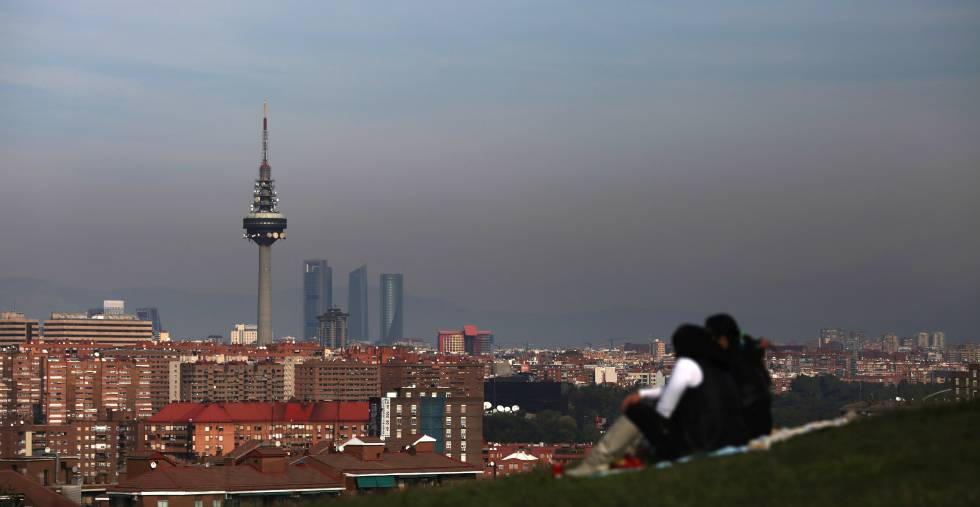
\includegraphics{Images/madrid.jpg}
\caption{title}
\end{figure}

\subsubsection{Objetivo}\label{objetivo}

El 30 de diciembre de 2016 el Ayuntamiento de Madrid empieza a
restringir el tráfico al centro de la ciudad mediante la aplicación del
escenario 3 del protocolo de contaminación. Esta fue la primera vez que
se aplicó un escenario tan restrictivo. Demuestra mediante
visualizaciones de datos que ha ocurrido después de ello. Para dicho
problema, haremos uso de un dataset con datos sobre la calidad del aire
en Madrid desde 2001. El dataset contiene un archivo csv por año. Dentro
de cada uno de ellos habrá medidas diarias de distintas estaciones.
Estas estaciones miden diferentes parámetros y no siempre todos se
registran en cada una de las estaciones.

Enlace dataset:
https://www.kaggle.com/decide-soluciones/air-quality-madrid/downloads/csvs\_per\_year.zip/5

    \paragraph{Librerias}\label{librerias}

    \begin{Verbatim}[commandchars=\\\{\}]
{\color{incolor}In [{\color{incolor}1}]:} \PY{k+kn}{import} \PY{n+nn}{pandas} \PY{k}{as} \PY{n+nn}{pd}
        \PY{k+kn}{import} \PY{n+nn}{os}
        \PY{k+kn}{import} \PY{n+nn}{glob}
        \PY{k+kn}{import} \PY{n+nn}{numpy} \PY{k}{as} \PY{n+nn}{np}
        \PY{k+kn}{import} \PY{n+nn}{matplotlib}\PY{n+nn}{.}\PY{n+nn}{pyplot} \PY{k}{as} \PY{n+nn}{plt}
        \PY{k+kn}{import} \PY{n+nn}{datetime} \PY{k}{as} \PY{n+nn}{dt}
        \PY{k+kn}{from} \PY{n+nn}{matplotlib}\PY{n+nn}{.}\PY{n+nn}{pyplot} \PY{k}{import} \PY{n}{cm}
        \PY{k+kn}{import} \PY{n+nn}{warnings}
        \PY{n}{warnings}\PY{o}{.}\PY{n}{filterwarnings}\PY{p}{(}\PY{l+s+s1}{\PYZsq{}}\PY{l+s+s1}{ignore}\PY{l+s+s1}{\PYZsq{}}\PY{p}{)}
\end{Verbatim}


    \subsection{Ejercicio 1}\label{ejercicio-1}

\paragraph{Lo primero que tendremos que hacer es cargar todos los
archivos csv en un mismo DataFrame para poder manipularlos. Habrá que
comprobar si existen datos redundantes o
anómalos.}\label{lo-primero-que-tendremos-que-hacer-es-cargar-todos-los-archivos-csv-en-un-mismo-dataframe-para-poder-manipularlos.-habruxe1-que-comprobar-si-existen-datos-redundantes-o-anuxf3malos.}

\paragraph{Para medir la calidad del aire de un día obtendremos el peor
valor de cada estación meteorológica ese día y después calcularemos la
media de estos. Con dicho valor se estimará como de buena es la calidad
teniendo en cuenta la siguiente tabla. Al final habrá que hacer una
transformación de valores continuos a
categóricos.}\label{para-medir-la-calidad-del-aire-de-un-duxeda-obtendremos-el-peor-valor-de-cada-estaciuxf3n-meteoroluxf3gica-ese-duxeda-y-despuuxe9s-calcularemos-la-media-de-estos.-con-dicho-valor-se-estimaruxe1-como-de-buena-es-la-calidad-teniendo-en-cuenta-la-siguiente-tabla.-al-final-habruxe1-que-hacer-una-transformaciuxf3n-de-valores-continuos-a-categuxf3ricos.}

\paragraph{Proporcionar dicha información en un DataFrame y luego
guardarlo en un archivo
csv.}\label{proporcionar-dicha-informaciuxf3n-en-un-dataframe-y-luego-guardarlo-en-un-archivo-csv.}

\begin{figure}
\centering
\includegraphics{attachment:Screenshot_1.png}
\caption{Screenshot\_1.png}
\end{figure}

    \paragraph{Funciones}\label{funciones}

    \begin{Verbatim}[commandchars=\\\{\}]
{\color{incolor}In [{\color{incolor}2}]:} \PY{c+c1}{\PYZsh{} Función para categorizar la media del aire.}
        \PY{k}{def} \PY{n+nf}{custom\PYZus{}categorical}\PY{p}{(}\PY{n}{valor}\PY{p}{)}\PY{p}{:}
            \PY{k}{if} \PY{n}{valor} \PY{o}{\PYZlt{}} \PY{l+m+mi}{49}\PY{p}{:}
                \PY{k}{return} \PY{l+m+mi}{1}
            \PY{k}{if} \PY{n}{valor} \PY{o}{\PYZlt{}} \PY{l+m+mi}{99}\PY{p}{:}
                \PY{k}{return} \PY{l+m+mi}{2}
            \PY{k}{if} \PY{n}{valor} \PY{o}{\PYZlt{}} \PY{l+m+mi}{150}\PY{p}{:}
                \PY{k}{return} \PY{l+m+mi}{3}
            \PY{k}{return} \PY{l+m+mi}{4}
\end{Verbatim}


    Primero tenemos que unir todos los ficheros de datos en uno solo.

    \begin{Verbatim}[commandchars=\\\{\}]
{\color{incolor}In [{\color{incolor}3}]:} \PY{c+c1}{\PYZsh{} Ruta de los ficheros.}
        \PY{n}{ruta} \PY{o}{=} \PY{l+s+s1}{\PYZsq{}}\PY{l+s+s1}{Datos/Original/}\PY{l+s+s1}{\PYZsq{}}
        
        \PY{c+c1}{\PYZsh{} Carga de los ficheros.}
        \PY{n}{ficheros} \PY{o}{=} \PY{n}{glob}\PY{o}{.}\PY{n}{glob}\PY{p}{(}\PY{n}{ruta} \PY{o}{+} \PY{l+s+s2}{\PYZdq{}}\PY{l+s+s2}{/*.csv}\PY{l+s+s2}{\PYZdq{}}\PY{p}{)}
        \PY{n}{Dataframe} \PY{o}{=} \PY{n}{pd}\PY{o}{.}\PY{n}{DataFrame}\PY{p}{(}\PY{p}{)}
        \PY{n}{lista\PYZus{}dataframe} \PY{o}{=} \PY{p}{[}\PY{p}{]}
        \PY{k}{for} \PY{n}{fichero} \PY{o+ow}{in} \PY{n}{ficheros}\PY{p}{:}
            \PY{n}{dataframe\PYZus{}temp} \PY{o}{=} \PY{n}{pd}\PY{o}{.}\PY{n}{read\PYZus{}csv}\PY{p}{(}\PY{n}{fichero}\PY{p}{,} \PY{n}{index\PYZus{}col}\PY{o}{=}\PY{l+m+mi}{0}\PY{p}{,} \PY{n}{header}\PY{o}{=}\PY{l+m+mi}{0}\PY{p}{)}
            \PY{n}{lista\PYZus{}dataframe}\PY{o}{.}\PY{n}{append}\PY{p}{(}\PY{n}{dataframe\PYZus{}temp}\PY{p}{)}
            
        \PY{c+c1}{\PYZsh{} Unión de los ficheros.}
        \PY{n}{Dataframe} \PY{o}{=} \PY{n}{pd}\PY{o}{.}\PY{n}{concat}\PY{p}{(}\PY{n}{lista\PYZus{}dataframe}\PY{p}{,} \PY{n}{sort}\PY{o}{=}\PY{k+kc}{False}\PY{p}{)}
        
        \PY{c+c1}{\PYZsh{} Guardamos el csv unido.}
        \PY{n}{Dataframe}\PY{o}{.}\PY{n}{to\PYZus{}csv}\PY{p}{(}\PY{l+s+s2}{\PYZdq{}}\PY{l+s+s2}{Datos/datos\PYZus{}unidos.csv}\PY{l+s+s2}{\PYZdq{}}\PY{p}{,} \PY{n}{encoding}\PY{o}{=}\PY{l+s+s2}{\PYZdq{}}\PY{l+s+s2}{ISO\PYZhy{}8859\PYZhy{}1}\PY{l+s+s2}{\PYZdq{}}\PY{p}{)}
        
        \PY{c+c1}{\PYZsh{} Contamos el número de registros del dataset.}
        \PY{n+nb}{print}\PY{p}{(}\PY{l+s+s2}{\PYZdq{}}\PY{l+s+s2}{Hay }\PY{l+s+s2}{\PYZdq{}} \PY{o}{+} \PY{n+nb}{str}\PY{p}{(}\PY{n+nb}{len}\PY{p}{(}\PY{n}{Dataframe}\PY{p}{)}\PY{p}{)} \PY{o}{+} \PY{l+s+s2}{\PYZdq{}}\PY{l+s+s2}{ registros}\PY{l+s+s2}{\PYZdq{}}\PY{p}{)}
\end{Verbatim}


    \begin{Verbatim}[commandchars=\\\{\}]
Hay 3808224 registros

    \end{Verbatim}

    Cargamos el fichero de datos unido y lo tratamos para limpiar y
organizar el dataset.

    \begin{Verbatim}[commandchars=\\\{\}]
{\color{incolor}In [{\color{incolor}4}]:} \PY{c+c1}{\PYZsh{} Carga del fichero de datos unido.}
        \PY{n}{Dataframe} \PY{o}{=} \PY{n}{pd}\PY{o}{.}\PY{n}{read\PYZus{}csv}\PY{p}{(}\PY{l+s+s2}{\PYZdq{}}\PY{l+s+s2}{Datos/datos\PYZus{}unidos.csv}\PY{l+s+s2}{\PYZdq{}}\PY{p}{,} \PY{n}{encoding}\PY{o}{=}\PY{l+s+s2}{\PYZdq{}}\PY{l+s+s2}{ISO\PYZhy{}8859\PYZhy{}1}\PY{l+s+s2}{\PYZdq{}}\PY{p}{)}
        
        \PY{c+c1}{\PYZsh{} Ordenación por fecha.}
        \PY{n}{Dataframe} \PY{o}{=} \PY{n}{Dataframe}\PY{o}{.}\PY{n}{sort\PYZus{}values}\PY{p}{(}\PY{n}{by}\PY{o}{=}\PY{l+s+s1}{\PYZsq{}}\PY{l+s+s1}{date}\PY{l+s+s1}{\PYZsq{}}\PY{p}{,} \PY{n}{ascending}\PY{o}{=}\PY{k+kc}{True}\PY{p}{)}
        
        \PY{c+c1}{\PYZsh{} Reseteo del índice.}
        \PY{n}{Dataframe} \PY{o}{=} \PY{n}{Dataframe}\PY{o}{.}\PY{n}{reset\PYZus{}index}\PY{p}{(}\PY{n}{drop}\PY{o}{=}\PY{k+kc}{True}\PY{p}{)}
        
        \PY{c+c1}{\PYZsh{} Redondeamos los datos 2 decimales.}
        \PY{n}{Dataframe} \PY{o}{=} \PY{n+nb}{round}\PY{p}{(}\PY{n}{Dataframe}\PY{p}{,} \PY{l+m+mi}{3}\PY{p}{)}
        
        \PY{c+c1}{\PYZsh{} Transformamos la columna \PYZsq{}date\PYZsq{} a datetime.}
        \PY{n}{Dataframe}\PY{p}{[}\PY{l+s+s2}{\PYZdq{}}\PY{l+s+s2}{date}\PY{l+s+s2}{\PYZdq{}}\PY{p}{]} \PY{o}{=} \PY{n}{pd}\PY{o}{.}\PY{n}{to\PYZus{}datetime}\PY{p}{(}\PY{n}{Dataframe}\PY{p}{[}\PY{l+s+s2}{\PYZdq{}}\PY{l+s+s2}{date}\PY{l+s+s2}{\PYZdq{}}\PY{p}{]}\PY{p}{)}
        
        \PY{c+c1}{\PYZsh{} Eliminamos la hora pues no la necesitamos para el estudio y así agrupamos mejor.}
        \PY{n}{Dataframe}\PY{p}{[}\PY{l+s+s2}{\PYZdq{}}\PY{l+s+s2}{date}\PY{l+s+s2}{\PYZdq{}}\PY{p}{]} \PY{o}{=} \PY{n}{Dataframe}\PY{p}{[}\PY{l+s+s2}{\PYZdq{}}\PY{l+s+s2}{date}\PY{l+s+s2}{\PYZdq{}}\PY{p}{]}\PY{o}{.}\PY{n}{dt}\PY{o}{.}\PY{n}{date}
        
        \PY{c+c1}{\PYZsh{} Transformamos de nuevo la columna \PYZsq{}date\PYZsq{} a datetime.}
        \PY{n}{Dataframe}\PY{p}{[}\PY{l+s+s2}{\PYZdq{}}\PY{l+s+s2}{date}\PY{l+s+s2}{\PYZdq{}}\PY{p}{]} \PY{o}{=} \PY{n}{pd}\PY{o}{.}\PY{n}{to\PYZus{}datetime}\PY{p}{(}\PY{n}{Dataframe}\PY{p}{[}\PY{l+s+s2}{\PYZdq{}}\PY{l+s+s2}{date}\PY{l+s+s2}{\PYZdq{}}\PY{p}{]}\PY{p}{)}
        
        \PY{c+c1}{\PYZsh{} Transformamos la estación a tipo string para poder sacar el máximo más fácilmente.}
        \PY{n}{Dataframe}\PY{p}{[}\PY{l+s+s2}{\PYZdq{}}\PY{l+s+s2}{station}\PY{l+s+s2}{\PYZdq{}}\PY{p}{]} \PY{o}{=} \PY{n}{Dataframe}\PY{p}{[}\PY{l+s+s1}{\PYZsq{}}\PY{l+s+s1}{station}\PY{l+s+s1}{\PYZsq{}}\PY{p}{]}\PY{o}{.}\PY{n}{astype}\PY{p}{(}\PY{n+nb}{str}\PY{p}{)}
        
        \PY{c+c1}{\PYZsh{} Calculamos el valor máximo de cada registro (fila).}
        \PY{n}{Dataframe}\PY{p}{[}\PY{l+s+s2}{\PYZdq{}}\PY{l+s+s2}{max}\PY{l+s+s2}{\PYZdq{}}\PY{p}{]} \PY{o}{=} \PY{n}{Dataframe}\PY{o}{.}\PY{n}{max}\PY{p}{(}\PY{n}{axis}\PY{o}{=}\PY{l+m+mi}{1}\PY{p}{,} \PY{n}{numeric\PYZus{}only}\PY{o}{=}\PY{k+kc}{True}\PY{p}{)}
        
        \PY{c+c1}{\PYZsh{} Guardamos el dataset.}
        \PY{n}{Dataframe}\PY{o}{.}\PY{n}{to\PYZus{}csv}\PY{p}{(}\PY{l+s+s2}{\PYZdq{}}\PY{l+s+s2}{Datos/datos\PYZus{}agrupados.csv}\PY{l+s+s2}{\PYZdq{}}\PY{p}{,} \PY{n}{encoding}\PY{o}{=}\PY{l+s+s2}{\PYZdq{}}\PY{l+s+s2}{ISO\PYZhy{}8859\PYZhy{}1}\PY{l+s+s2}{\PYZdq{}}\PY{p}{)}
        
        \PY{c+c1}{\PYZsh{} Mostramos los 10 primeros.}
        \PY{n}{Dataframe}\PY{o}{.}\PY{n}{head}\PY{p}{(}\PY{l+m+mi}{10}\PY{p}{)}
\end{Verbatim}


\begin{Verbatim}[commandchars=\\\{\}]
{\color{outcolor}Out[{\color{outcolor}4}]:}         date   BEN    CO   EBE   MXY  NMHC   NO\_2     NOx   OXY    O\_3   PM10  \textbackslash{}
        0 2001-01-01   NaN  1.45   NaN   NaN   NaN  50.39  159.70   NaN   4.18  21.22   
        1 2001-01-01  3.23  1.25  2.56  4.58  0.24  55.29  120.00  2.22   7.83  30.56   
        2 2001-01-01  2.13  0.87  1.44  3.16   NaN  53.40  100.00  1.06   8.35  36.67   
        3 2001-01-01  0.40  0.79   NaN  2.09  0.14  47.32   54.95  1.17   3.40  14.44   
        4 2001-01-01  1.08  0.67  0.96   NaN  0.10  43.82   68.61   NaN  32.49  11.89   
        5 2001-01-01  3.00  1.55   NaN   NaN   NaN  55.27  126.70   NaN   6.23  19.61   
        6 2001-01-01   NaN  0.92   NaN   NaN   NaN  55.16  117.00   NaN   4.99  18.20   
        7 2001-01-01   NaN  1.12   NaN   NaN   NaN  81.36  117.20   NaN  12.89  27.47   
        8 2001-01-01   NaN  3.62   NaN   NaN  0.79  59.15  283.90   NaN   7.44  40.14   
        9 2001-01-01   NaN  1.23   NaN   NaN   NaN  55.75  127.20   NaN   8.38  44.95   
        
           PM25   PXY   SO\_2   TCH    TOL   station  CH4  NO     max  
        0   NaN   NaN  10.86   NaN    NaN  28079019  NaN NaN  159.70  
        1   NaN  1.80  22.10  1.58  10.74  28079099  NaN NaN  120.00  
        2   NaN  1.28  11.42   NaN   7.04  28079025  NaN NaN  100.00  
        3   NaN  0.86   9.69  1.51   5.83  28079024  NaN NaN   54.95  
        4   NaN   NaN   9.35  1.42   4.49  28079023  NaN NaN   68.61  
        5   NaN   NaN  27.27   NaN   7.79  28079022  NaN NaN  126.70  
        6   NaN   NaN  32.52   NaN    NaN  28079021  NaN NaN  117.00  
        7   NaN   NaN  15.82   NaN    NaN  28079036  NaN NaN  117.20  
        8   NaN   NaN  23.39  2.15    NaN  28079018  NaN NaN  283.90  
        9   NaN   NaN  14.56   NaN    NaN  28079017  NaN NaN  127.20  
\end{Verbatim}
            
    Ya tenemos el dataset con el campo 'date' sin la hora, los datos
redondeados a 2 decimales y con el máximo valor de cada fila en una
nueva columna 'max'.

    Seguimos limpiando y organizando el dataset para obtener la calidad del
aire media medida por una estación en cada día.

    \begin{Verbatim}[commandchars=\\\{\}]
{\color{incolor}In [{\color{incolor}5}]:} \PY{n+nb}{print}\PY{p}{(}\PY{l+s+s2}{\PYZdq{}}\PY{l+s+s2}{Hay: }\PY{l+s+s2}{\PYZdq{}} \PY{o}{+} \PY{n+nb}{str}\PY{p}{(}\PY{n+nb}{len}\PY{p}{(}\PY{n}{Dataframe}\PY{p}{[}\PY{n}{Dataframe}\PY{p}{[}\PY{l+s+s2}{\PYZdq{}}\PY{l+s+s2}{max}\PY{l+s+s2}{\PYZdq{}}\PY{p}{]} \PY{o}{!=} \PY{n}{Dataframe}\PY{p}{[}\PY{l+s+s2}{\PYZdq{}}\PY{l+s+s2}{max}\PY{l+s+s2}{\PYZdq{}}\PY{p}{]}\PY{p}{]}\PY{p}{)}\PY{p}{)} \PY{o}{+} \PY{l+s+s2}{\PYZdq{}}\PY{l+s+s2}{ columnas todo a NaN.}\PY{l+s+s2}{\PYZdq{}}\PY{p}{)}
        
        \PY{c+c1}{\PYZsh{} Eliminamos los registros cuyas filas de datos están todos a NaN y reseteamos el índice.}
        \PY{n}{Dataframe} \PY{o}{=} \PY{n}{Dataframe}\PY{o}{.}\PY{n}{drop}\PY{p}{(}\PY{n}{Dataframe}\PY{p}{[}\PY{n}{Dataframe}\PY{p}{[}\PY{l+s+s2}{\PYZdq{}}\PY{l+s+s2}{max}\PY{l+s+s2}{\PYZdq{}}\PY{p}{]} \PY{o}{!=} \PY{n}{Dataframe}\PY{p}{[}\PY{l+s+s2}{\PYZdq{}}\PY{l+s+s2}{max}\PY{l+s+s2}{\PYZdq{}}\PY{p}{]}\PY{p}{]}\PY{o}{.}\PY{n}{index}\PY{p}{)}
        
        \PY{c+c1}{\PYZsh{} Reseteo del índice.}
        \PY{n}{Dataframe} \PY{o}{=} \PY{n}{Dataframe}\PY{o}{.}\PY{n}{reset\PYZus{}index}\PY{p}{(}\PY{n}{drop}\PY{o}{=}\PY{k+kc}{True}\PY{p}{)}
        
        \PY{n+nb}{print}\PY{p}{(}\PY{l+s+s2}{\PYZdq{}}\PY{l+s+s2}{Quedan: }\PY{l+s+s2}{\PYZdq{}} \PY{o}{+} \PY{n+nb}{str}\PY{p}{(}\PY{n+nb}{len}\PY{p}{(}\PY{n}{Dataframe}\PY{p}{[}\PY{n}{Dataframe}\PY{p}{[}\PY{l+s+s2}{\PYZdq{}}\PY{l+s+s2}{max}\PY{l+s+s2}{\PYZdq{}}\PY{p}{]} \PY{o}{!=} \PY{n}{Dataframe}\PY{p}{[}\PY{l+s+s2}{\PYZdq{}}\PY{l+s+s2}{max}\PY{l+s+s2}{\PYZdq{}}\PY{p}{]}\PY{p}{]}\PY{p}{)}\PY{p}{)} \PY{o}{+} \PY{l+s+s2}{\PYZdq{}}\PY{l+s+s2}{ columnas todo a NaN.}\PY{l+s+s2}{\PYZdq{}}\PY{p}{)}
        
        \PY{c+c1}{\PYZsh{} Agrupamos por estación y fecha (día concreto) para sacar la media de máximos valores medidos.}
        \PY{n}{Dataframe} \PY{o}{=} \PY{n}{Dataframe}\PY{o}{.}\PY{n}{groupby}\PY{p}{(}\PY{p}{[}\PY{l+s+s2}{\PYZdq{}}\PY{l+s+s2}{station}\PY{l+s+s2}{\PYZdq{}}\PY{p}{,} \PY{l+s+s2}{\PYZdq{}}\PY{l+s+s2}{date}\PY{l+s+s2}{\PYZdq{}}\PY{p}{]}\PY{p}{)}\PY{p}{[}\PY{l+s+s1}{\PYZsq{}}\PY{l+s+s1}{max}\PY{l+s+s1}{\PYZsq{}}\PY{p}{]}\PY{o}{.}\PY{n}{mean}\PY{p}{(}\PY{p}{)}
        
        \PY{c+c1}{\PYZsh{} Reseteamos el índice.}
        \PY{n}{Dataframe} \PY{o}{=} \PY{n}{Dataframe}\PY{o}{.}\PY{n}{reset\PYZus{}index}\PY{p}{(}\PY{p}{)}
        
        \PY{c+c1}{\PYZsh{} Guardamos el dataset.}
        \PY{n}{Dataframe}\PY{o}{.}\PY{n}{to\PYZus{}csv}\PY{p}{(}\PY{l+s+s2}{\PYZdq{}}\PY{l+s+s2}{Datos/datos\PYZus{}preprocesados.csv}\PY{l+s+s2}{\PYZdq{}}\PY{p}{,} \PY{n}{encoding}\PY{o}{=}\PY{l+s+s2}{\PYZdq{}}\PY{l+s+s2}{ISO\PYZhy{}8859\PYZhy{}1}\PY{l+s+s2}{\PYZdq{}}\PY{p}{)}
        
        \PY{c+c1}{\PYZsh{} Mostramos los 10 primeros.}
        \PY{n}{Dataframe}\PY{o}{.}\PY{n}{head}\PY{p}{(}\PY{l+m+mi}{10}\PY{p}{)}
\end{Verbatim}


    \begin{Verbatim}[commandchars=\\\{\}]
Hay: 13346 columnas todo a NaN.
Quedan: 0 columnas todo a NaN.

    \end{Verbatim}

\begin{Verbatim}[commandchars=\\\{\}]
{\color{outcolor}Out[{\color{outcolor}5}]:}     station       date         max
        0  28079001 2001-01-02  169.500000
        1  28079001 2001-01-03  173.284583
        2  28079001 2001-01-04  154.293333
        3  28079001 2001-01-05  210.120833
        4  28079001 2001-01-06  127.873750
        5  28079001 2001-01-07  141.195417
        6  28079001 2001-01-08  240.280417
        7  28079001 2001-01-09  211.216667
        8  28079001 2001-01-10  269.662500
        9  28079001 2001-01-11  192.406250
\end{Verbatim}
            
    Ahora ya tenemos el dataset libre de filas a NaN y con la media de los
perores valores medidos por una estación a lo largo de un día (realiza
una medición cada hora).

    \subsection{Ejercicio 2}\label{ejercicio-2}

\paragraph{Explica visualmente como se distribuyen las calidades del
aire entre buena, admisible, mala y muy mala. Realiza para ello un pie
chart. Que se puede concluir de dicho
gráfico.}\label{explica-visualmente-como-se-distribuyen-las-calidades-del-aire-entre-buena-admisible-mala-y-muy-mala.-realiza-para-ello-un-pie-chart.-que-se-puede-concluir-de-dicho-gruxe1fico.}

    \begin{Verbatim}[commandchars=\\\{\}]
{\color{incolor}In [{\color{incolor}6}]:} \PY{c+c1}{\PYZsh{} Carga del fichero de datos unido.}
        \PY{n}{Dataframe} \PY{o}{=} \PY{n}{pd}\PY{o}{.}\PY{n}{read\PYZus{}csv}\PY{p}{(}\PY{l+s+s2}{\PYZdq{}}\PY{l+s+s2}{Datos/datos\PYZus{}preprocesados.csv}\PY{l+s+s2}{\PYZdq{}}\PY{p}{,} \PY{n}{encoding}\PY{o}{=}\PY{l+s+s2}{\PYZdq{}}\PY{l+s+s2}{ISO\PYZhy{}8859\PYZhy{}1}\PY{l+s+s2}{\PYZdq{}}\PY{p}{,} \PY{n}{index\PYZus{}col}\PY{o}{=}\PY{l+m+mi}{0}\PY{p}{)}
        
        \PY{c+c1}{\PYZsh{} Sacamos la media de los peores valores medidos a lo largo de un día por todas las estaciones.}
        \PY{n}{Dataframe} \PY{o}{=} \PY{n}{Dataframe}\PY{o}{.}\PY{n}{groupby}\PY{p}{(}\PY{l+s+s2}{\PYZdq{}}\PY{l+s+s2}{date}\PY{l+s+s2}{\PYZdq{}}\PY{p}{)}\PY{p}{[}\PY{l+s+s1}{\PYZsq{}}\PY{l+s+s1}{max}\PY{l+s+s1}{\PYZsq{}}\PY{p}{]}\PY{o}{.}\PY{n}{mean}\PY{p}{(}\PY{p}{)}
        
        \PY{c+c1}{\PYZsh{} Reseteamos el índice.}
        \PY{n}{Dataframe} \PY{o}{=} \PY{n}{Dataframe}\PY{o}{.}\PY{n}{reset\PYZus{}index}\PY{p}{(}\PY{p}{)}
        
        \PY{c+c1}{\PYZsh{} Guardamos el dataset.}
        \PY{n}{Dataframe}\PY{o}{.}\PY{n}{to\PYZus{}csv}\PY{p}{(}\PY{l+s+s2}{\PYZdq{}}\PY{l+s+s2}{Datos/datos\PYZus{}media\PYZus{}dia.csv}\PY{l+s+s2}{\PYZdq{}}\PY{p}{,} \PY{n}{encoding}\PY{o}{=}\PY{l+s+s2}{\PYZdq{}}\PY{l+s+s2}{ISO\PYZhy{}8859\PYZhy{}1}\PY{l+s+s2}{\PYZdq{}}\PY{p}{)}
        
        \PY{c+c1}{\PYZsh{} Categorización del valor medio del aire para un día.}
        \PY{n}{valores} \PY{o}{=} \PY{n}{Dataframe}\PY{p}{[}\PY{l+s+s1}{\PYZsq{}}\PY{l+s+s1}{max}\PY{l+s+s1}{\PYZsq{}}\PY{p}{]}\PY{o}{.}\PY{n}{apply}\PY{p}{(}\PY{k}{lambda} \PY{n}{x}\PY{p}{:} \PY{n}{custom\PYZus{}categorical}\PY{p}{(}\PY{n}{x}\PY{p}{)}\PY{p}{)}
        
        \PY{c+c1}{\PYZsh{} Preparamos las listas para el pie chart.}
        \PY{n}{unique}\PY{p}{,} \PY{n}{counts} \PY{o}{=} \PY{n}{np}\PY{o}{.}\PY{n}{unique}\PY{p}{(}\PY{n}{valores}\PY{p}{,} \PY{n}{return\PYZus{}counts}\PY{o}{=}\PY{k+kc}{True}\PY{p}{)}
        
        \PY{c+c1}{\PYZsh{} Mostramos los datos calculados.}
        \PY{n+nb}{print}\PY{p}{(}\PY{n+nb}{dict}\PY{p}{(}\PY{n+nb}{zip}\PY{p}{(}\PY{n}{unique}\PY{p}{,} \PY{n}{counts}\PY{p}{)}\PY{p}{)}\PY{p}{)}
        
        \PY{c+c1}{\PYZsh{} Etiquetas.}
        \PY{n}{etiquetas} \PY{o}{=} \PY{n}{np}\PY{o}{.}\PY{n}{array}\PY{p}{(}\PY{n}{unique}\PY{p}{)}\PY{o}{.}\PY{n}{astype}\PY{p}{(}\PY{l+s+s1}{\PYZsq{}}\PY{l+s+s1}{U}\PY{l+s+s1}{\PYZsq{}}\PY{p}{)} 
        \PY{n}{etiquetas}\PY{p}{[}\PY{n}{etiquetas} \PY{o}{==} \PY{l+s+s2}{\PYZdq{}}\PY{l+s+s2}{1}\PY{l+s+s2}{\PYZdq{}}\PY{p}{]} \PY{o}{=} \PY{l+s+s2}{\PYZdq{}}\PY{l+s+s2}{Buena}\PY{l+s+s2}{\PYZdq{}}
        \PY{n}{etiquetas}\PY{p}{[}\PY{n}{etiquetas} \PY{o}{==} \PY{l+s+s2}{\PYZdq{}}\PY{l+s+s2}{2}\PY{l+s+s2}{\PYZdq{}}\PY{p}{]} \PY{o}{=} \PY{l+s+s2}{\PYZdq{}}\PY{l+s+s2}{Admisible}\PY{l+s+s2}{\PYZdq{}}
        \PY{n}{etiquetas}\PY{p}{[}\PY{n}{etiquetas} \PY{o}{==} \PY{l+s+s2}{\PYZdq{}}\PY{l+s+s2}{3}\PY{l+s+s2}{\PYZdq{}}\PY{p}{]} \PY{o}{=} \PY{l+s+s2}{\PYZdq{}}\PY{l+s+s2}{Mala}\PY{l+s+s2}{\PYZdq{}}
        \PY{n}{etiquetas}\PY{p}{[}\PY{n}{etiquetas} \PY{o}{==} \PY{l+s+s2}{\PYZdq{}}\PY{l+s+s2}{4}\PY{l+s+s2}{\PYZdq{}}\PY{p}{]} \PY{o}{=} \PY{l+s+s2}{\PYZdq{}}\PY{l+s+s2}{Muy mala}\PY{l+s+s2}{\PYZdq{}}
        
        \PY{c+c1}{\PYZsh{} Colores}
        \PY{n}{colores} \PY{o}{=} \PY{n}{np}\PY{o}{.}\PY{n}{copy}\PY{p}{(}\PY{n}{etiquetas}\PY{p}{)}
        \PY{n}{colores}\PY{p}{[}\PY{n}{colores} \PY{o}{==} \PY{l+s+s2}{\PYZdq{}}\PY{l+s+s2}{Buena}\PY{l+s+s2}{\PYZdq{}}\PY{p}{]} \PY{o}{=} \PY{l+s+s2}{\PYZdq{}}\PY{l+s+s2}{Green}\PY{l+s+s2}{\PYZdq{}}
        \PY{n}{colores}\PY{p}{[}\PY{n}{colores} \PY{o}{==} \PY{l+s+s2}{\PYZdq{}}\PY{l+s+s2}{Admisible}\PY{l+s+s2}{\PYZdq{}}\PY{p}{]} \PY{o}{=} \PY{l+s+s2}{\PYZdq{}}\PY{l+s+s2}{Yellow}\PY{l+s+s2}{\PYZdq{}}
        \PY{n}{colores}\PY{p}{[}\PY{n}{colores} \PY{o}{==} \PY{l+s+s2}{\PYZdq{}}\PY{l+s+s2}{Mala}\PY{l+s+s2}{\PYZdq{}}\PY{p}{]} \PY{o}{=} \PY{l+s+s2}{\PYZdq{}}\PY{l+s+s2}{Red}\PY{l+s+s2}{\PYZdq{}}
        \PY{n}{colores}\PY{p}{[}\PY{n}{colores} \PY{o}{==} \PY{l+s+s2}{\PYZdq{}}\PY{l+s+s2}{Muy mala}\PY{l+s+s2}{\PYZdq{}}\PY{p}{]} \PY{o}{=} \PY{l+s+s2}{\PYZdq{}}\PY{l+s+s2}{Brown}\PY{l+s+s2}{\PYZdq{}}
        
        \PY{n+nb}{print}\PY{p}{(}\PY{n}{etiquetas}\PY{p}{)}
        
        \PY{c+c1}{\PYZsh{} Mostramos la gráfica.}
        \PY{n}{fig}\PY{p}{,} \PY{n}{ax} \PY{o}{=} \PY{n}{plt}\PY{o}{.}\PY{n}{subplots}\PY{p}{(}\PY{n}{figsize}\PY{o}{=}\PY{p}{(}\PY{l+m+mi}{20}\PY{p}{,} \PY{l+m+mi}{10}\PY{p}{)}\PY{p}{)}
        \PY{n}{ax}\PY{o}{.}\PY{n}{pie}\PY{p}{(}\PY{n}{counts}\PY{p}{,} \PY{n}{labels}\PY{o}{=}\PY{n}{etiquetas}\PY{p}{,} \PY{n}{autopct}\PY{o}{=}\PY{l+s+s1}{\PYZsq{}}\PY{l+s+si}{\PYZpc{}1.1f}\PY{l+s+si}{\PYZpc{}\PYZpc{}}\PY{l+s+s1}{\PYZsq{}}\PY{p}{,} \PY{n}{shadow}\PY{o}{=}\PY{k+kc}{True}\PY{p}{,} \PY{n}{startangle}\PY{o}{=}\PY{l+m+mi}{90}\PY{p}{,} \PY{n}{colors}\PY{o}{=}\PY{n}{colores}\PY{p}{)}
        \PY{n}{ax}\PY{o}{.}\PY{n}{axis}\PY{p}{(}\PY{l+s+s1}{\PYZsq{}}\PY{l+s+s1}{equal}\PY{l+s+s1}{\PYZsq{}}\PY{p}{)}  
        \PY{n}{plt}\PY{o}{.}\PY{n}{title}\PY{p}{(}\PY{l+s+s2}{\PYZdq{}}\PY{l+s+s2}{Calidades del aire}\PY{l+s+s2}{\PYZdq{}}\PY{p}{)}
        \PY{n}{plt}\PY{o}{.}\PY{n}{show}\PY{p}{(}\PY{p}{)}
\end{Verbatim}


    \begin{Verbatim}[commandchars=\\\{\}]
\{1: 598, 2: 3490, 3: 1468, 4: 774\}
['Buena' 'Admisible' 'Mala' 'Muy mala']

    \end{Verbatim}

    \begin{center}
    \adjustimage{max size={0.9\linewidth}{0.9\paperheight}}{output_15_1.png}
    \end{center}
    { \hspace*{\fill} \\}
    
    El aire de Madrid es admisible más de la mitad de los días, es malo o
muy malo un tercio de los días y tan solo una décima parte de los días
el aire es bueno.

    \subsection{Ejercicio 3}\label{ejercicio-3}

\paragraph{Una vez obtenida la calidad del aire para cada día, calcula
la calidad media de cada mes para que sea más fácil saber si la
contaminación ha disminuido desde que se restringió el acceso al centro
de Madrid. Explica visualmente si los protocolos de restricciones de
tráfico han tenido éxito. Utiliza para ello un diagrama de barras.
¿Podemos encontrar la diferencia entre lo que ocurría antes de aplicar
el protocolo y
después?}\label{una-vez-obtenida-la-calidad-del-aire-para-cada-duxeda-calcula-la-calidad-media-de-cada-mes-para-que-sea-muxe1s-fuxe1cil-saber-si-la-contaminaciuxf3n-ha-disminuido-desde-que-se-restringiuxf3-el-acceso-al-centro-de-madrid.-explica-visualmente-si-los-protocolos-de-restricciones-de-truxe1fico-han-tenido-uxe9xito.-utiliza-para-ello-un-diagrama-de-barras.-podemos-encontrar-la-diferencia-entre-lo-que-ocurruxeda-antes-de-aplicar-el-protocolo-y-despuuxe9s}

    Para ello, creamos un diagrama de barras indicando los meses pre y post
restricción.

    \begin{Verbatim}[commandchars=\\\{\}]
{\color{incolor}In [{\color{incolor}7}]:} \PY{c+c1}{\PYZsh{} Leemos el fichero de datos.}
        \PY{n}{Dataframe} \PY{o}{=} \PY{n}{pd}\PY{o}{.}\PY{n}{read\PYZus{}csv}\PY{p}{(}\PY{l+s+s2}{\PYZdq{}}\PY{l+s+s2}{Datos/datos\PYZus{}media\PYZus{}dia.csv}\PY{l+s+s2}{\PYZdq{}}\PY{p}{,} \PY{n}{encoding}\PY{o}{=}\PY{l+s+s2}{\PYZdq{}}\PY{l+s+s2}{ISO\PYZhy{}8859\PYZhy{}1}\PY{l+s+s2}{\PYZdq{}}\PY{p}{,} \PY{n}{index\PYZus{}col}\PY{o}{=}\PY{l+m+mi}{0}\PY{p}{)}
        
        \PY{c+c1}{\PYZsh{} Transformamos la columna \PYZsq{}date\PYZsq{} a datetime.}
        \PY{n}{Dataframe}\PY{p}{[}\PY{l+s+s2}{\PYZdq{}}\PY{l+s+s2}{date}\PY{l+s+s2}{\PYZdq{}}\PY{p}{]} \PY{o}{=} \PY{n}{pd}\PY{o}{.}\PY{n}{to\PYZus{}datetime}\PY{p}{(}\PY{n}{Dataframe}\PY{p}{[}\PY{l+s+s2}{\PYZdq{}}\PY{l+s+s2}{date}\PY{l+s+s2}{\PYZdq{}}\PY{p}{]}\PY{p}{)}
        
        \PY{c+c1}{\PYZsh{} Creamos los dataframes para antes y después de la restricción y el auxiliar (Dataframe\PYZus{}Mes).}
        \PY{n}{Dataframe\PYZus{}Mes} \PY{o}{=} \PY{n}{pd}\PY{o}{.}\PY{n}{DataFrame}\PY{p}{(}\PY{p}{)}
        \PY{n}{Dataframe\PYZus{}Post\PYZus{}Restriccion} \PY{o}{=} \PY{n}{pd}\PY{o}{.}\PY{n}{DataFrame}\PY{p}{(}\PY{p}{)} 
        \PY{n}{Dataframe\PYZus{}Pre\PYZus{}Restriccion} \PY{o}{=} \PY{n}{pd}\PY{o}{.}\PY{n}{DataFrame}\PY{p}{(}\PY{p}{)} 
        
        \PY{c+c1}{\PYZsh{} Agregamos las columnas de \PYZsq{}year\PYZsq{}, \PYZsq{}month\PYZsq{} y \PYZsq{}mean\PYZsq{}. }
        \PY{n}{Dataframe\PYZus{}Mes}\PY{p}{[}\PY{l+s+s2}{\PYZdq{}}\PY{l+s+s2}{year}\PY{l+s+s2}{\PYZdq{}}\PY{p}{]} \PY{o}{=} \PY{n}{Dataframe}\PY{p}{[}\PY{l+s+s2}{\PYZdq{}}\PY{l+s+s2}{date}\PY{l+s+s2}{\PYZdq{}}\PY{p}{]}\PY{o}{.}\PY{n}{dt}\PY{o}{.}\PY{n}{year}
        \PY{n}{Dataframe\PYZus{}Mes}\PY{p}{[}\PY{l+s+s2}{\PYZdq{}}\PY{l+s+s2}{month}\PY{l+s+s2}{\PYZdq{}}\PY{p}{]} \PY{o}{=} \PY{n}{Dataframe}\PY{p}{[}\PY{l+s+s2}{\PYZdq{}}\PY{l+s+s2}{date}\PY{l+s+s2}{\PYZdq{}}\PY{p}{]}\PY{o}{.}\PY{n}{dt}\PY{o}{.}\PY{n}{month}
        \PY{n}{Dataframe\PYZus{}Mes}\PY{p}{[}\PY{l+s+s2}{\PYZdq{}}\PY{l+s+s2}{mean}\PY{l+s+s2}{\PYZdq{}}\PY{p}{]} \PY{o}{=} \PY{n}{Dataframe}\PY{p}{[}\PY{l+s+s2}{\PYZdq{}}\PY{l+s+s2}{max}\PY{l+s+s2}{\PYZdq{}}\PY{p}{]}
        
        \PY{c+c1}{\PYZsh{} Agrupamos por mes y reseteamos el índice.}
        \PY{n}{Dataframe\PYZus{}Mes} \PY{o}{=} \PY{n+nb}{round}\PY{p}{(}\PY{n}{Dataframe\PYZus{}Mes}\PY{o}{.}\PY{n}{groupby}\PY{p}{(}\PY{p}{[}\PY{l+s+s2}{\PYZdq{}}\PY{l+s+s2}{year}\PY{l+s+s2}{\PYZdq{}}\PY{p}{,} \PY{l+s+s2}{\PYZdq{}}\PY{l+s+s2}{month}\PY{l+s+s2}{\PYZdq{}}\PY{p}{]}\PY{p}{)}\PY{o}{.}\PY{n}{mean}\PY{p}{(}\PY{p}{)}\PY{p}{,} \PY{l+m+mi}{1}\PY{p}{)}
        \PY{n}{Dataframe\PYZus{}Mes} \PY{o}{=} \PY{n}{Dataframe\PYZus{}Mes}\PY{o}{.}\PY{n}{reset\PYZus{}index}\PY{p}{(}\PY{p}{)}
        
        \PY{c+c1}{\PYZsh{} Dividimos el dataset por año antes y después de la restricción.}
        \PY{n}{Dataframe\PYZus{}Pre\PYZus{}Restriccion} \PY{o}{=} \PY{n}{Dataframe\PYZus{}Mes}\PY{p}{[}\PY{n}{Dataframe\PYZus{}Mes}\PY{p}{[}\PY{l+s+s2}{\PYZdq{}}\PY{l+s+s2}{year}\PY{l+s+s2}{\PYZdq{}}\PY{p}{]} \PY{o}{\PYZlt{}} \PY{l+m+mi}{2017}\PY{p}{]}
        \PY{n}{Dataframe\PYZus{}Post\PYZus{}Restriccion} \PY{o}{=} \PY{n}{Dataframe\PYZus{}Mes}\PY{p}{[}\PY{n}{Dataframe\PYZus{}Mes}\PY{p}{[}\PY{l+s+s2}{\PYZdq{}}\PY{l+s+s2}{year}\PY{l+s+s2}{\PYZdq{}}\PY{p}{]} \PY{o}{\PYZgt{}} \PY{l+m+mi}{2016}\PY{p}{]}
        
        \PY{c+c1}{\PYZsh{} Agrupamos por mes, sacamos la media y redondeamos a 3 decimales y reseteamos el índice.}
        \PY{n}{Dataframe\PYZus{}Post\PYZus{}Restriccion} \PY{o}{=} \PY{n+nb}{round}\PY{p}{(}\PY{n}{Dataframe\PYZus{}Post\PYZus{}Restriccion}\PY{o}{.}\PY{n}{groupby}\PY{p}{(}\PY{p}{[}\PY{l+s+s2}{\PYZdq{}}\PY{l+s+s2}{month}\PY{l+s+s2}{\PYZdq{}}\PY{p}{]}\PY{p}{)}\PY{o}{.}\PY{n}{mean}\PY{p}{(}\PY{p}{)}\PY{p}{,} \PY{l+m+mi}{3}\PY{p}{)}
        \PY{n}{Dataframe\PYZus{}Post\PYZus{}Restriccion} \PY{o}{=} \PY{n}{Dataframe\PYZus{}Post\PYZus{}Restriccion}\PY{o}{.}\PY{n}{reset\PYZus{}index}\PY{p}{(}\PY{p}{)}
        \PY{n}{Dataframe\PYZus{}Pre\PYZus{}Restriccion} \PY{o}{=} \PY{n+nb}{round}\PY{p}{(}\PY{n}{Dataframe\PYZus{}Pre\PYZus{}Restriccion}\PY{o}{.}\PY{n}{groupby}\PY{p}{(}\PY{p}{[}\PY{l+s+s2}{\PYZdq{}}\PY{l+s+s2}{month}\PY{l+s+s2}{\PYZdq{}}\PY{p}{]}\PY{p}{)}\PY{o}{.}\PY{n}{mean}\PY{p}{(}\PY{p}{)}\PY{p}{,} \PY{l+m+mi}{3}\PY{p}{)}
        \PY{n}{Dataframe\PYZus{}Pre\PYZus{}Restriccion} \PY{o}{=} \PY{n}{Dataframe\PYZus{}Pre\PYZus{}Restriccion}\PY{o}{.}\PY{n}{reset\PYZus{}index}\PY{p}{(}\PY{p}{)}
\end{Verbatim}


    Preparamos la gráfica.

    \begin{Verbatim}[commandchars=\\\{\}]
{\color{incolor}In [{\color{incolor}8}]:} \PY{c+c1}{\PYZsh{} Obtenemos la lista de valores a representar.}
        \PY{n}{media\PYZus{}calidad\PYZus{}pre\PYZus{}restriccion} \PY{o}{=} \PY{n}{Dataframe\PYZus{}Pre\PYZus{}Restriccion}\PY{p}{[}\PY{l+s+s2}{\PYZdq{}}\PY{l+s+s2}{mean}\PY{l+s+s2}{\PYZdq{}}\PY{p}{]}
        \PY{n}{media\PYZus{}calidad\PYZus{}post\PYZus{}restriccion} \PY{o}{=} \PY{n}{Dataframe\PYZus{}Post\PYZus{}Restriccion}\PY{p}{[}\PY{l+s+s2}{\PYZdq{}}\PY{l+s+s2}{mean}\PY{l+s+s2}{\PYZdq{}}\PY{p}{]}
        
        \PY{c+c1}{\PYZsh{} Preparamos la gráfica.}
        \PY{n}{ind} \PY{o}{=} \PY{n}{np}\PY{o}{.}\PY{n}{arange}\PY{p}{(}\PY{n+nb}{len}\PY{p}{(}\PY{n}{media\PYZus{}calidad\PYZus{}pre\PYZus{}restriccion}\PY{p}{)}\PY{p}{)}
        \PY{n}{ancho} \PY{o}{=} \PY{l+m+mf}{0.35}
        
        \PY{n}{fig}\PY{p}{,} \PY{n}{ax} \PY{o}{=} \PY{n}{plt}\PY{o}{.}\PY{n}{subplots}\PY{p}{(}\PY{n}{figsize}\PY{o}{=}\PY{p}{(}\PY{l+m+mi}{20}\PY{p}{,} \PY{l+m+mi}{10}\PY{p}{)}\PY{p}{)}
        \PY{n}{rects1} \PY{o}{=} \PY{n}{ax}\PY{o}{.}\PY{n}{bar}\PY{p}{(}\PY{n}{ind} \PY{o}{\PYZhy{}} \PY{n}{ancho}\PY{o}{/}\PY{l+m+mi}{2}\PY{p}{,} \PY{n}{media\PYZus{}calidad\PYZus{}pre\PYZus{}restriccion}\PY{p}{,} \PY{n}{ancho}\PY{p}{,} \PY{n}{color}\PY{o}{=}\PY{l+s+s1}{\PYZsq{}}\PY{l+s+s1}{SkyBlue}\PY{l+s+s1}{\PYZsq{}}\PY{p}{,} \PY{n}{label}\PY{o}{=}\PY{l+s+s1}{\PYZsq{}}\PY{l+s+s1}{Pre restricción}\PY{l+s+s1}{\PYZsq{}}\PY{p}{)}
        \PY{n}{rects2} \PY{o}{=} \PY{n}{ax}\PY{o}{.}\PY{n}{bar}\PY{p}{(}\PY{n}{ind} \PY{o}{+} \PY{n}{ancho}\PY{o}{/}\PY{l+m+mi}{2}\PY{p}{,} \PY{n}{media\PYZus{}calidad\PYZus{}post\PYZus{}restriccion}\PY{p}{,} \PY{n}{ancho}\PY{p}{,} \PY{n}{color}\PY{o}{=}\PY{l+s+s1}{\PYZsq{}}\PY{l+s+s1}{IndianRed}\PY{l+s+s1}{\PYZsq{}}\PY{p}{,} \PY{n}{label}\PY{o}{=}\PY{l+s+s1}{\PYZsq{}}\PY{l+s+s1}{Post restricción}\PY{l+s+s1}{\PYZsq{}}\PY{p}{)}
        
        \PY{n}{ax}\PY{o}{.}\PY{n}{set\PYZus{}ylabel}\PY{p}{(}\PY{l+s+s1}{\PYZsq{}}\PY{l+s+s1}{Calidad del aire}\PY{l+s+s1}{\PYZsq{}}\PY{p}{)}
        \PY{n}{ax}\PY{o}{.}\PY{n}{set\PYZus{}title}\PY{p}{(}\PY{l+s+s1}{\PYZsq{}}\PY{l+s+s1}{Calidad del aire por mes}\PY{l+s+s1}{\PYZsq{}}\PY{p}{)}
        \PY{n}{ax}\PY{o}{.}\PY{n}{set\PYZus{}xticks}\PY{p}{(}\PY{n}{ind}\PY{p}{)}
        \PY{n}{ax}\PY{o}{.}\PY{n}{set\PYZus{}xticklabels}\PY{p}{(}\PY{p}{(}\PY{l+s+s1}{\PYZsq{}}\PY{l+s+s1}{Enero}\PY{l+s+s1}{\PYZsq{}}\PY{p}{,} \PY{l+s+s1}{\PYZsq{}}\PY{l+s+s1}{Febrero}\PY{l+s+s1}{\PYZsq{}}\PY{p}{,} \PY{l+s+s1}{\PYZsq{}}\PY{l+s+s1}{Marzo}\PY{l+s+s1}{\PYZsq{}}\PY{p}{,} \PY{l+s+s1}{\PYZsq{}}\PY{l+s+s1}{Abril}\PY{l+s+s1}{\PYZsq{}}\PY{p}{,} \PY{l+s+s1}{\PYZsq{}}\PY{l+s+s1}{Mayo}\PY{l+s+s1}{\PYZsq{}}\PY{p}{,} \PY{l+s+s1}{\PYZsq{}}\PY{l+s+s1}{Junio}\PY{l+s+s1}{\PYZsq{}}\PY{p}{,} \PY{l+s+s1}{\PYZsq{}}\PY{l+s+s1}{Julio}\PY{l+s+s1}{\PYZsq{}}\PY{p}{,} \PY{l+s+s1}{\PYZsq{}}\PY{l+s+s1}{Agostp}\PY{l+s+s1}{\PYZsq{}}\PY{p}{,} \PY{l+s+s1}{\PYZsq{}}\PY{l+s+s1}{Septiembre}\PY{l+s+s1}{\PYZsq{}}\PY{p}{,} \PYZbs{}
                            \PY{l+s+s1}{\PYZsq{}}\PY{l+s+s1}{Octubre}\PY{l+s+s1}{\PYZsq{}}\PY{p}{,} \PY{l+s+s1}{\PYZsq{}}\PY{l+s+s1}{Noviembre}\PY{l+s+s1}{\PYZsq{}}\PY{p}{,} \PY{l+s+s1}{\PYZsq{}}\PY{l+s+s1}{Diciembre}\PY{l+s+s1}{\PYZsq{}} \PY{p}{)}\PY{p}{)}
        \PY{n}{ax}\PY{o}{.}\PY{n}{legend}\PY{p}{(}\PY{p}{)}
        
        \PY{c+c1}{\PYZsh{} Funciópn para pintar en la gráfica los distintos valores}
        \PY{k}{def} \PY{n+nf}{autolabel}\PY{p}{(}\PY{n}{rects}\PY{p}{,} \PY{n}{xpos}\PY{o}{=}\PY{l+s+s1}{\PYZsq{}}\PY{l+s+s1}{center}\PY{l+s+s1}{\PYZsq{}}\PY{p}{)}\PY{p}{:}
            \PY{n}{xpos} \PY{o}{=} \PY{n}{xpos}\PY{o}{.}\PY{n}{lower}\PY{p}{(}\PY{p}{)} 
            \PY{n}{ha} \PY{o}{=} \PY{p}{\PYZob{}}\PY{l+s+s1}{\PYZsq{}}\PY{l+s+s1}{center}\PY{l+s+s1}{\PYZsq{}}\PY{p}{:} \PY{l+s+s1}{\PYZsq{}}\PY{l+s+s1}{center}\PY{l+s+s1}{\PYZsq{}}\PY{p}{,} \PY{l+s+s1}{\PYZsq{}}\PY{l+s+s1}{right}\PY{l+s+s1}{\PYZsq{}}\PY{p}{:} \PY{l+s+s1}{\PYZsq{}}\PY{l+s+s1}{left}\PY{l+s+s1}{\PYZsq{}}\PY{p}{,} \PY{l+s+s1}{\PYZsq{}}\PY{l+s+s1}{left}\PY{l+s+s1}{\PYZsq{}}\PY{p}{:} \PY{l+s+s1}{\PYZsq{}}\PY{l+s+s1}{right}\PY{l+s+s1}{\PYZsq{}}\PY{p}{\PYZcb{}}
            \PY{n}{offset} \PY{o}{=} \PY{p}{\PYZob{}}\PY{l+s+s1}{\PYZsq{}}\PY{l+s+s1}{center}\PY{l+s+s1}{\PYZsq{}}\PY{p}{:} \PY{l+m+mf}{0.5}\PY{p}{,} \PY{l+s+s1}{\PYZsq{}}\PY{l+s+s1}{right}\PY{l+s+s1}{\PYZsq{}}\PY{p}{:} \PY{l+m+mf}{0.57}\PY{p}{,} \PY{l+s+s1}{\PYZsq{}}\PY{l+s+s1}{left}\PY{l+s+s1}{\PYZsq{}}\PY{p}{:} \PY{l+m+mf}{0.43}\PY{p}{\PYZcb{}}
        
            \PY{k}{for} \PY{n}{rect} \PY{o+ow}{in} \PY{n}{rects}\PY{p}{:}
                \PY{n}{height} \PY{o}{=} \PY{n}{rect}\PY{o}{.}\PY{n}{get\PYZus{}height}\PY{p}{(}\PY{p}{)}
                \PY{n}{ax}\PY{o}{.}\PY{n}{text}\PY{p}{(}\PY{n}{rect}\PY{o}{.}\PY{n}{get\PYZus{}x}\PY{p}{(}\PY{p}{)} \PY{o}{+} \PY{n}{rect}\PY{o}{.}\PY{n}{get\PYZus{}width}\PY{p}{(}\PY{p}{)}\PY{o}{*}\PY{n}{offset}\PY{p}{[}\PY{n}{xpos}\PY{p}{]}\PY{p}{,} \PY{l+m+mf}{1.01}\PY{o}{*}\PY{n}{height}\PY{p}{,}
                        \PY{l+s+s1}{\PYZsq{}}\PY{l+s+si}{\PYZob{}\PYZcb{}}\PY{l+s+s1}{\PYZsq{}}\PY{o}{.}\PY{n}{format}\PY{p}{(}\PY{n}{height}\PY{p}{)}\PY{p}{,} \PY{n}{ha}\PY{o}{=}\PY{n}{ha}\PY{p}{[}\PY{n}{xpos}\PY{p}{]}\PY{p}{,} \PY{n}{va}\PY{o}{=}\PY{l+s+s1}{\PYZsq{}}\PY{l+s+s1}{bottom}\PY{l+s+s1}{\PYZsq{}}\PY{p}{)}
        
        
        \PY{n}{autolabel}\PY{p}{(}\PY{n}{rects1}\PY{p}{,} \PY{l+s+s2}{\PYZdq{}}\PY{l+s+s2}{left}\PY{l+s+s2}{\PYZdq{}}\PY{p}{)}
        \PY{n}{autolabel}\PY{p}{(}\PY{n}{rects2}\PY{p}{,} \PY{l+s+s2}{\PYZdq{}}\PY{l+s+s2}{right}\PY{l+s+s2}{\PYZdq{}}\PY{p}{)}
        
        \PY{c+c1}{\PYZsh{} Mostramos la gráfica.}
        \PY{n}{plt}\PY{o}{.}\PY{n}{show}\PY{p}{(}\PY{p}{)}
\end{Verbatim}


    \begin{center}
    \adjustimage{max size={0.9\linewidth}{0.9\paperheight}}{output_21_0.png}
    \end{center}
    { \hspace*{\fill} \\}
    
    Observando la gráfica podemos afirmar que en la mayoría de meses la
restricción ha funcionado salvo en los meses finales del año cuyos datos
son especialmente malos (en especial Noviembre del 2017). Esto puede
deberse a otros factores climáticos (falta de lluvia, ausencia de
viento, cambios en la humedad relativa del aire, etc.) que hayan
propiciado la acumulación de contaminación atmosférica, factores de los
cuales no hay datos incluidos en el dataset. 

    \paragraph{Por último, queremos tratar de entender los cambios de la
calidad del aire en estos últimos años. Obtén un diagrama de cajas donde
cada caja corresponda a un año y haz una interpretación de los
resultados.}\label{por-uxfaltimo-queremos-tratar-de-entender-los-cambios-de-la-calidad-del-aire-en-estos-uxfaltimos-auxf1os.-obtuxe9n-un-diagrama-de-cajas-donde-cada-caja-corresponda-a-un-auxf1o-y-haz-una-interpretaciuxf3n-de-los-resultados.}

    \begin{Verbatim}[commandchars=\\\{\}]
{\color{incolor}In [{\color{incolor}9}]:} \PY{n}{Dataframe\PYZus{}Mes}\PY{o}{.}\PY{n}{boxplot}\PY{p}{(}\PY{n}{column}\PY{o}{=}\PY{l+s+s1}{\PYZsq{}}\PY{l+s+s1}{mean}\PY{l+s+s1}{\PYZsq{}}\PY{p}{,} \PY{n}{by}\PY{o}{=}\PY{l+s+s1}{\PYZsq{}}\PY{l+s+s1}{year}\PY{l+s+s1}{\PYZsq{}}\PY{p}{,} \PY{n}{figsize}\PY{o}{=}\PY{p}{(}\PY{l+m+mi}{20}\PY{p}{,}\PY{l+m+mi}{10}\PY{p}{)}\PY{p}{)}
\end{Verbatim}


\begin{Verbatim}[commandchars=\\\{\}]
{\color{outcolor}Out[{\color{outcolor}9}]:} <matplotlib.axes.\_subplots.AxesSubplot at 0x15de1b1d0>
\end{Verbatim}
            
    \begin{center}
    \adjustimage{max size={0.9\linewidth}{0.9\paperheight}}{output_24_1.png}
    \end{center}
    { \hspace*{\fill} \\}
    
    Observando la gráfica se aprecia una tendencia en la mejora de la
calidad del aire y en los valores que se compactan desde 2001 hasta 2012
donde se estabilizan (exceptuando algún valor atípico). \\
En 2017 y 2018, se ven valores más altos y dispersos. Con el diagrama de
barras anterior podemos justificar los valores especialmente altos y la
dispersión alta de 2017 en base a los últimos 3 meses de 2017 (sobretodo
Noviembre). Para poder obtener conclusiones con relación al año 2018, se
necesitaría que estuvieran todos sus datos completados.


    % Add a bibliography block to the postdoc
    
    
    
    \end{document}
